\documentclass[crop,tikz]{standalone}
\usetikzlibrary{positioning,arrows,fit,calc}
\pgfdeclarelayer{bg}
\pgfsetlayers{bg,main}
\tikzset{
	>=stealth'
}
\begin{document}
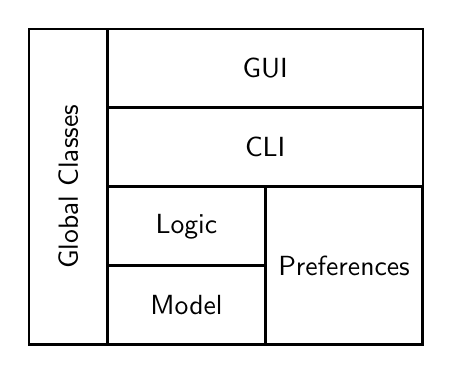
\begin{tikzpicture}[
node distance = -0.1mm,
every node/.style = {
	font = \sffamily
},
jar/.style = {
	draw,
	minimum height = 2.cm
},
package/.style = {
	draw,
	minimum height = 1.3cm,
	minimum width = 1.5cm
},
class/.style = {
	draw,
	fill = white,
	minimum height = \baselineskip,
	minimum width = .5cm
}
]

\node (global) [draw, thick, minimum height = 1cm, minimum width = 4.01cm, rotate=90] {Global Classes};
\node (model) [draw, thick, right = -0.25mm of global.south west, anchor = south west, minimum height = 1cm, minimum width = 2cm] {Model};
\node (logic) [draw, thick, above = -0.25mm of model.north west, anchor = south west, minimum height = 1cm, minimum width = 1.995cm] {Logic};
\node (pref) [draw, thick, right = -0.25mm of model.south east, anchor=south west, minimum height = 2cm, minimum width = 1.995cm] {Preferences};
\node (cli) [draw, thick, above = -0.25mm of logic.north west, anchor= south west, minimum height = 1cm, minimum width = 4cm] {CLI};
\node (gui) [draw, thick, above = -0.25mm of cli.north west, anchor = south west, minimum height = 1cm, minimum width = 4cm] {GUI};

\end{tikzpicture}

\end{document}